\documentclass[12pt]{article}
\usepackage[utf8]{inputenc}
\usepackage[margin=1in]{geometry}
\usepackage{amsmath}\usepackage{amssymb}\usepackage{multicol}\usepackage{enumitem}
\usepackage{pgfplots}\pgfplotsset{compat=1.17}
\setlength{\parindent}{0pt}
\begin{document}

\fbox{\parbox{0.97\linewidth}{\small\textbf{Final answers} (record here --- graded on the answer; show your work):\\[6pt]1.~\underline{\hspace{1.5cm}}\quad 2.~\underline{\hspace{1.5cm}}\quad 3.~\underline{\hspace{1.5cm}}\quad 4.~\underline{\hspace{1.5cm}}\quad 5.~\underline{\hspace{1.5cm}}\quad 6.~\underline{\hspace{1.5cm}}\quad 7.~\underline{\hspace{1.5cm}}\quad 8.~\underline{\hspace{1.5cm}}\quad 9.~\underline{\hspace{1.5cm}}}}
\vspace{0.35cm}

\begin{center}{\Large \textbf{Mixed Practice: Vertex Form and Graphing}}\end{center}\vspace{0.2cm}
% Mixed Practice: Vertex Form and Graphing
\textbf{Example (Mixed Practice: Vertex Form and Graphing):}

For $y=2(x-1)^2-3$: vertex $(1,-3)$, opens up; y-intercept $y=2(0-1)^2-3=-1$, point $(0,-1)$, mirror point $(2,-1)$.

\vspace{0.2cm}\hrule\vspace{0.35cm}
\textbf{Directions: For each function, find the vertex, direction of opening, y-intercept, and its mirror point.}

\begin{multicols}{2}
\begin{enumerate}[label=\textbf{\arabic*.}, start=1, itemsep=2cm]
  \item $\displaystyle y=(x+2)^2-1$
  \item $\displaystyle y=-3(x-1)^2+4$
  \item $\displaystyle y=\frac{1}{2}(x-4)^2+2$
  \item $\displaystyle y=-(x+3)^2+2$
\end{enumerate}
\end{multicols}
\vspace{0.25cm}\hrule\vspace{0.35cm}

\begin{center}{\Large \textbf{Mixed Practice: Transformations and Max/Min}}\end{center}\vspace{0.2cm}
% Mixed Practice: Transformations and Max/Min
\textbf{Example (Mixed Practice: Transformations and Max/Min):}

For $y=-(x+4)^2+7$: transformations are shift left 4, reflect over x-axis, shift up 7; since $a=-1<0$, maximum value is $7$ at $x=-4$.

\begin{center}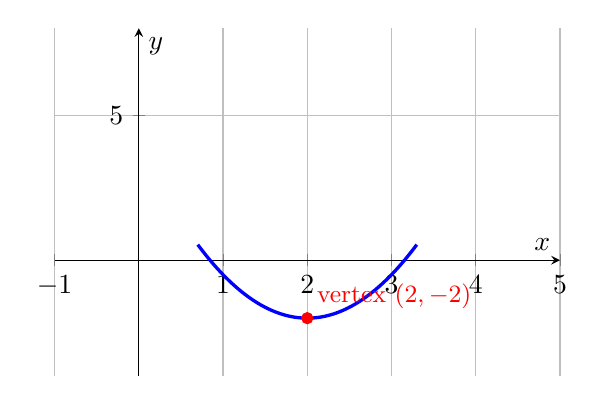
\begin{tikzpicture}
\begin{axis}[axis lines=middle,xlabel=$x$,ylabel=$y$,xmin=-1,xmax=5,ymin=-4,ymax=8,width=8cm,height=6cm,grid=both,samples=80]
\addplot[very thick,blue,domain=0.7:3.3]{1.5*(x-2)^2-2};
\addplot[only marks,mark=*,red] coordinates {(2,-2)};
\node[above right,red,font=\small] at (axis cs:2,-2) {vertex $(2,-2)$};
\end{axis}\end{tikzpicture}\end{center}
{\small\centering Reference graph of $y=1.5(x-2)^2-2$.\par}
\vspace{0.2cm}\hrule\vspace{0.35cm}
\textbf{Directions: Describe the transformations from $y=x^2$ and state the max/min value for each function.}

\begin{multicols}{2}
\begin{enumerate}[label=\textbf{\arabic*.}, start=5, itemsep=3cm]
  \item $y=1.5(x-2)^2-2$ (use the graph above to confirm the vertex)
  \item $\displaystyle y=-2(x+1)^2+5$
  \item $\displaystyle y=3(x-2)^2-1$
  \item A ball's height is $h(t)=-16t^2+32t+4$. Find the maximum height and when it occurs.
\end{enumerate}
\end{multicols}

\vspace{0.2cm}\hrule\vspace{0.3cm}
\textbf{Challenge} (same sheet):\\[4pt]
\begin{enumerate}[label=\textbf{\arabic*.}, start=9, itemsep=2.2cm]
  \item Create your own vertex-form equation with a maximum value of $10$ at $x=-2$, and describe all its transformations from $y=x^2$.
\end{enumerate}

\newpage

\begin{center}{\Large \textbf{Answer Key --- fully worked}}\end{center}
\vspace{0.25cm}
\textbf{Procedure:} Identify $a$, $h$, and $k$ from the equation.; State the vertex, direction of opening, and axis of symmetry.; Find the y-intercept by substituting $x=0$, and its mirror point across the axis of symmetry.; Describe the transformations from $y=x^2$: shifts, reflection, stretch/compression.; State the max/min value ($k$) and where it occurs ($x=h$), interpreting units for word problems..\\[8pt]
\begin{enumerate}[label=\textbf{\arabic*.},itemsep=7pt]
  \item Vertex $(-2,-1)$, opens up; y-intercept $y=(0+2)^2-1=3$, point $(0,3)$, mirror point $(-4,3)$.
  \item Vertex $(1,4)$, opens down; y-intercept $y=-3(0-1)^2+4=1$, point $(0,1)$, mirror point $(2,1)$.
  \item Vertex $(4,2)$, opens up; y-intercept $y=\frac{1}{2}(0-4)^2+2=10$, point $(0,10)$, mirror point $(8,10)$.
  \item Vertex $(-3,2)$, opens down; y-intercept $y=-(0+3)^2+2=-7$, point $(0,-7)$, mirror point $(-6,-7)$.
  \item Shift right 2, stretch narrower by 1.5, shift down 2; vertex $(2,-2)$, minimum value $-2$ -- matches the graph shown.
  \item Shift left 1, reflect over x-axis, stretch narrower by 2, shift up 5; maximum value $5$ at $x=-1$.
  \item Shift right 2, stretch narrower by 3, shift down 1; vertex $(2,-1)$, minimum value $-1$.
  \item $t=-\frac{32}{-32}=1$; $h(1)=-16+32+4=20$. Maximum height is 20 feet, occurring at 1 second.
  \item A maximum value of $10$ at $x=-2$ means the vertex is $(-2,10)$ with $a<0$, so $h=-2$, $k=10$. One valid answer: $y=-(x+2)^2+10$. Transformations from $y=x^2$: shift left 2, reflect over the x-axis, shift up 10 (any $a<0$ works, e.g. $y=-3(x+2)^2+10$ would also add a narrowing stretch by 3).
\end{enumerate}

\end{document}